\chapter{Prezentacja warstwy użytkowej projektu}
\label{chap:prezentacja}
\section{Wprowadzenie}
W tym rozdziale zostanie przedstawiona warstwa użytkowa projektu, która obejmuje interfejs graficzny aplikacji oraz sposób interakcji użytkownika z systemem. Warstwa ta została zaprojektowana z myślą o intuicyjności i łatwości obsługi, co jest kluczowe dla zapewnienia pozytywnego doświadczenia użytkownika.

\section{Ekran logowania i rejestracji}
Ekran logowania jest pierwszym krokiem, z jakim spotyka się użytkownik po uruchomieniu aplikacji. Umożliwia on zalogowanie się na istniejące konto lub rejestrację nowego użytkownika. Interfejs jest prosty i przejrzysty, co pozwala na szybkie wprowadzenie danych.
\begin{figure}[H]
    \centering
    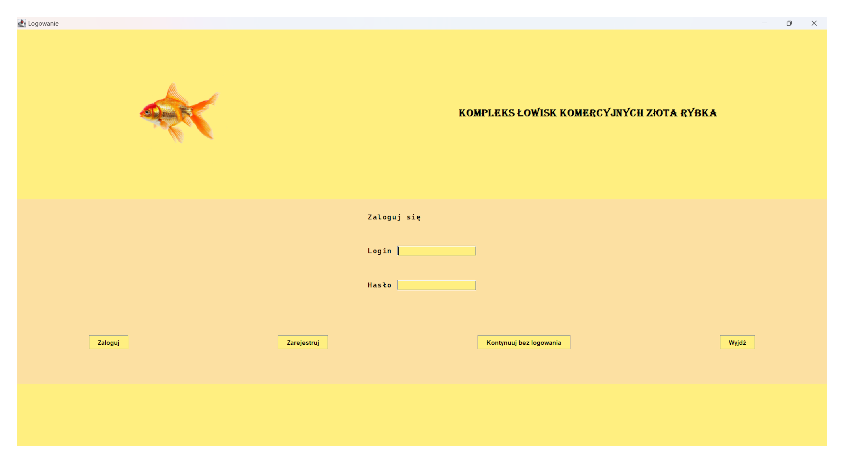
\includegraphics[width=0.8\linewidth]{figures/login.eps}
    \caption{Ekran logowania.}
    \label{fig:login_screen}
    \small{Źródło: Opracowane przy użyciu Java Swing}
\end{figure}
\clearpage

\section{Ekran rejestracji}
Ekran rejestracji pozwala na tworzenie nowych kont użytkowników. Użytkownik musi wprowadzić swoje dane, takie jak nazwa użytkownika, hasło i adres e-mail. Po poprawnym wypełnieniu formularza, użytkownik może zalogować się do aplikacji.
\begin{figure}[H]
    \centering
    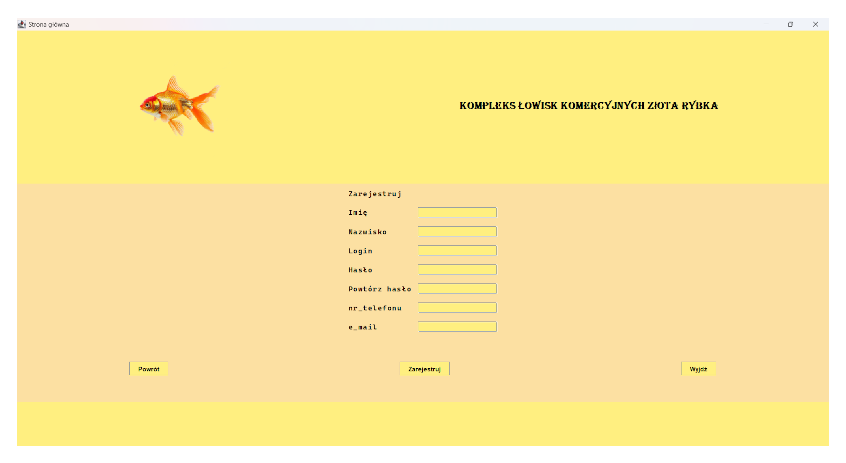
\includegraphics[width=0.8\linewidth]{figures/register.eps}
    \caption{Ekran rejestracji.}
    \label{fig:register_screen}
    \small{Źródło: Opracowane przy użyciu Java Swing}
\end{figure}
\clearpage

\section{Ekran po zalogowaniu}
Po zalogowaniu użytkownik zostaje przekierowany do głównego menu aplikacji, gdzie może przeglądać dostępne usługi, takie jak rezerwacja łowisk, wędek i domków. Interfejs jest zaprojektowany w sposób umożliwiający łatwe nawigowanie między różnymi funkcjami.
\begin{figure}[H]
    \centering
    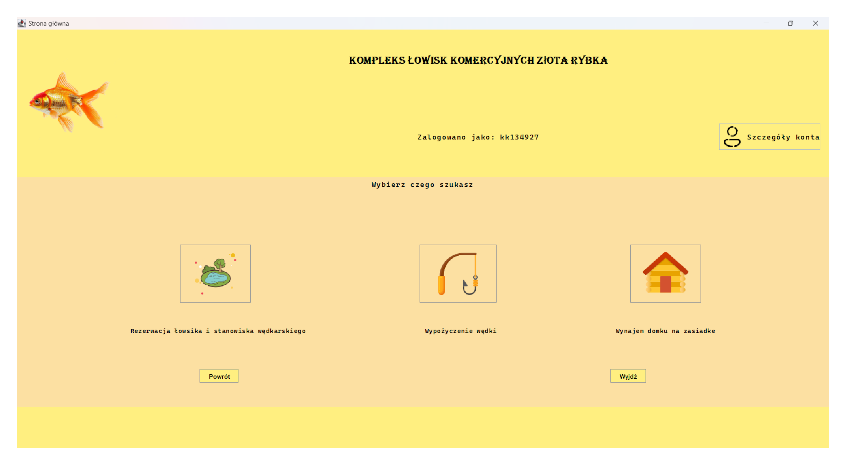
\includegraphics[width=0.8\linewidth]{figures/after.eps}
    \caption{Ekran po zalogowaniu.}
    \label{fig:after_login_screen}
    \small{Źródło: Opracowane przy użyciu Java Swing}\
\end{figure}
\clearpage

\section{Ekran bez logowania}
Ekran bez logowania umożliwia przeglądanie dostępnych usług bez konieczności logowania się. Rózni się też tym że z racji że sie nie logujemy to zamiast loginu w Zalogowano jako: wyświetla się Gość. Użytkownik może zobaczyć listę łowisk, wędek i domków, ale nie ma możliwości dokonywania rezerwacji ani przeglądania historii rezerwacji.
\begin{figure}[H]
    \centering
    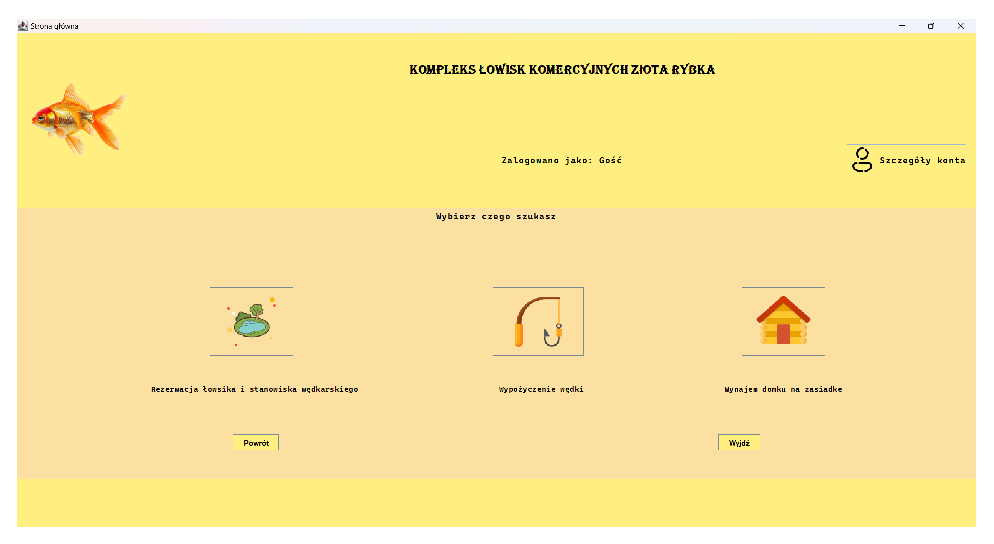
\includegraphics[width=0.8\linewidth]{figures/without.eps}
    \caption{Ekran bez logowania.}
    \label{fig:without_login_screen}
    \small{Źródło: Opracowane przy użyciu Java Swing}
\end{figure}
\clearpage

\section{Ekran rezerwacji łowisk}
Ekran rezerwacji łowiska umożliwia użytkownikowi dokonanie rezerwacji na wybrane łowisko. Użytkownik może wybrać datę rozpoczęcia i zakończenia rezerwacji.
\begin{figure}[H]
    \centering
    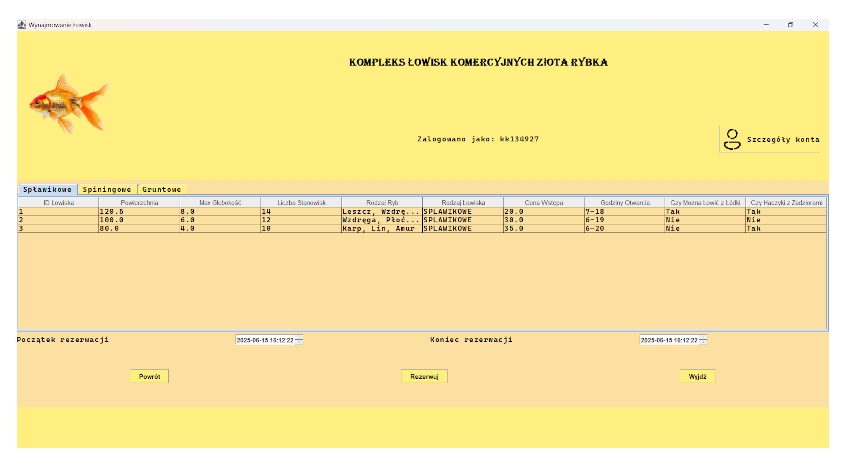
\includegraphics[width=0.8\linewidth]{figures/lakes.eps}
    \caption{Ekran rezerwacji łowisk.}
    \label{fig:lakes_screen}
    \small{Źródło: Opracowane przy użyciu Java Swing}
\end{figure}
\clearpage

\section{Ekran rezerwacji wędek}
Ekran rezerwacji wędek pozwala użytkownikowi na wybór dostępnych wędek do rezerwacji. Użytkownik może przeglądać dostępne modele i dokonać rezerwacji na wybraną wędkę.
\begin{figure}[H]
    \centering
    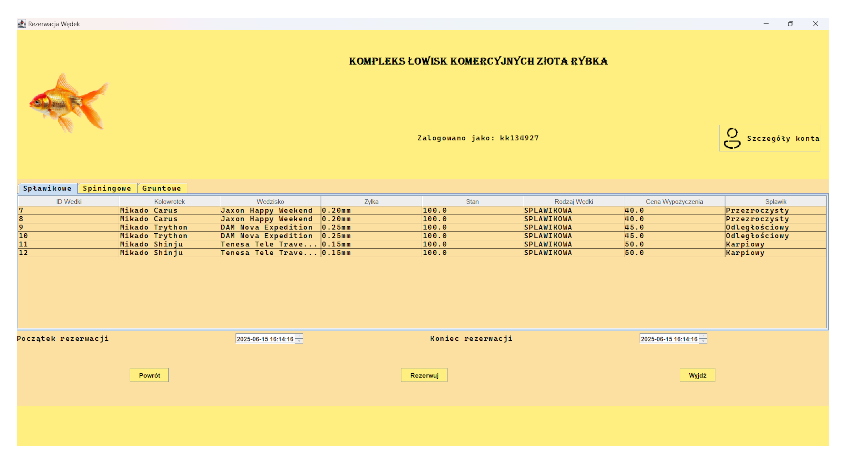
\includegraphics[width=0.8\linewidth]{figures/rods.eps}
    \caption{Ekran rezerwacji wędek.}
    \label{fig:rods_screen}
    \small{Źródło: Opracowane przy użyciu Java Swing}
\end{figure}
\clearpage

\section{Ekran rezerwacji domków}
Ekran rezerwacji domków umożliwia użytkownikowi dokonanie rezerwacji na wybrany domek. Użytkownik może przeglądać dostępne domki, sprawdzać ich dostępność i dokonywać rezerwacji.
\begin{figure}[H]
    \centering
    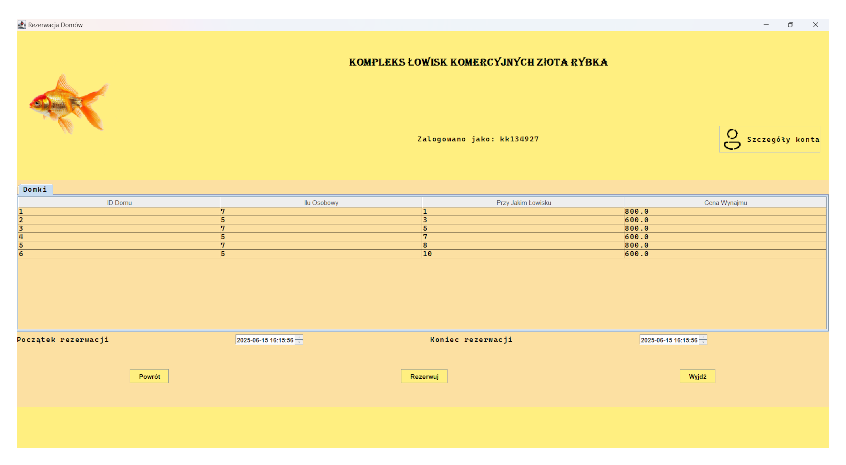
\includegraphics[width=0.8\linewidth]{figures/houses.eps}
    \caption{Ekran rezerwacji domków.}
    \label{fig:houses_screen}
    \small{Źródło: Opracowane przy użyciu Java Swing}
\end{figure}
\clearpage

\section{Ekran historia rezerwacji}
Ekran historii rezerwacji pozwala użytkownikowi na przeglądanie wszystkich dokonanych rezerwacji. Użytkownik może zobaczyć szczegóły każdej rezerwacji, takie jak daty, koszty i rodzaje usług.
\begin{figure}[H]
    \centering
    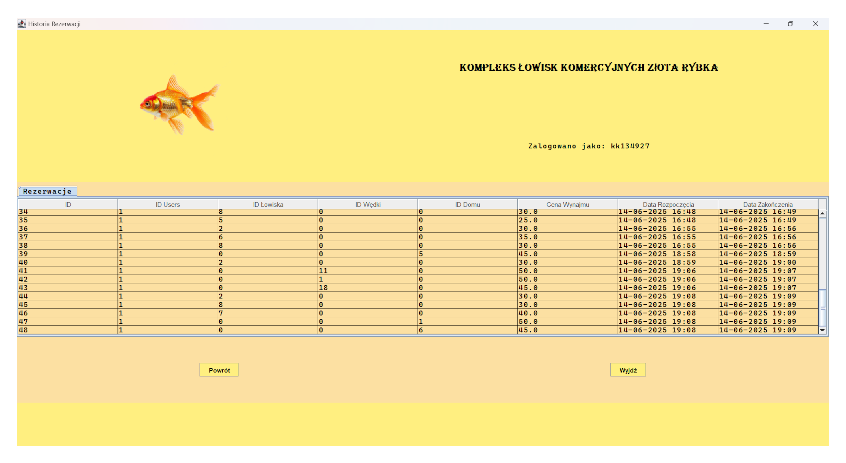
\includegraphics[width=0.8\linewidth]{figures/history.eps}
    \caption{Ekran historii rezerwacji.}
    \label{fig:history_screen}
    \small{Źródło: Opracowane przy użyciu Java Swing}
\end{figure}
\clearpage


